De meeste datacenters zijn uitgerust met 19\inch-kasten waarin 19\inch-servers hangen

\begin{figure}[h!]
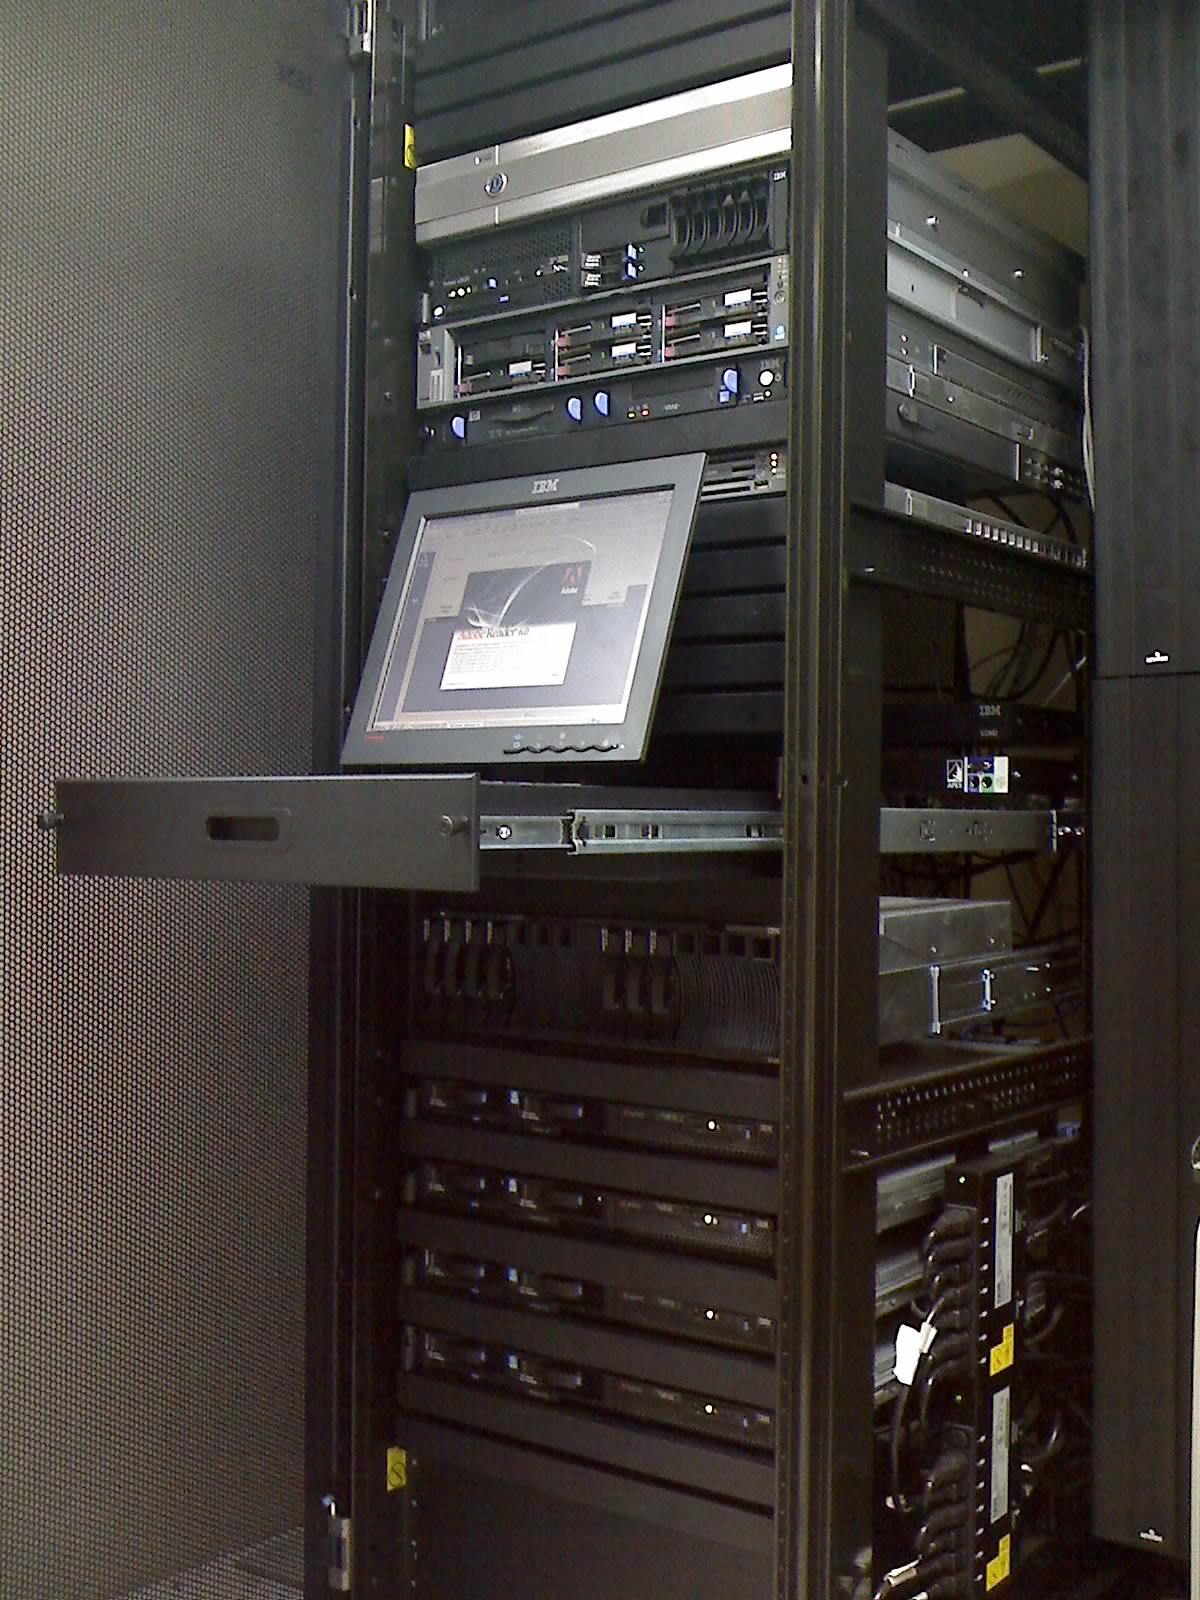
\includegraphics[width=0.75\linewidth]{Wiki_Rack001.jpg}
\caption Foto van Jfreyre afkomstig van \url{https://commons.wikimedia.org/wiki/File:Rack001.jpg}
\centering
\end{figure}

Om hogere dichtheden te bereiken wordt er gebruik gemaakt van blade servers. Bij blade servers zitten er meedere servers (blades) in \'e\'en fysieke behuizing (19\inch-kast). De servers delen een backplane, de voeding(en) en de behuizing waardoor er effectief meer servers passen op dezelfde oppervlakte. Een nadeel van blades is wel dat de warmte ontwikkeling ook veel meer geconcentreerd wordt en dat kan leiden tot zogenaamde hotspots, wat slecht is voor de koeling.
